\documentclass[11pt]{article}
\usepackage[margin=1in]{geometry}                % See geometry.pdf to learn the layout options. There are lots.
\geometry{letterpaper}                   % ... or a4paper or a5paper or ... 
%\geometry{landscape}                % Activate for for rotated page geometry
%\usepackage[parfill]{parskip}    % Activate to begin paragraphs with an empty line rather than an indent
\usepackage{color}
\definecolor{myblue}{rgb}{0.0, 0.0, 0.85}
\usepackage[breaklinks=true, colorlinks=true, linkcolor=red, urlcolor=myblue, citecolor=black]{hyperref}
\urlstyle{rm}
\usepackage{mathptmx}
\usepackage{graphicx}
\usepackage{amssymb}
\usepackage{epstopdf}
\usepackage{sidecap}
\usepackage{authblk}
\usepackage{booktabs}
\usepackage[font=small,labelfont=bf]{caption}
\usepackage{enumitem}
\usepackage{wrapfig}
%\usepackage{draftwatermark}
%\SetWatermarkText{DRAFT}
%\SetWatermarkScale{1.2}
%\SetWatermarkColor[gray]{0.85}
\DeclareGraphicsRule{.tif}{png}{.png}{`convert #1 `dirname #1`/`basename #1 .tif`.png}
\pagestyle{plain}

\def\bfr{\bf\color{red}}
\def\bfp{\color{magenta}}
\def\geohub{{\tt geohub}}
\def\resp{respectively}
\def\selah{SELAH}
\def\nch{718}
\def\nh{957\pm94}
\def\dh{10\%\pm9\%}
\def\nce{389}
\def\ne{556\pm83}
\def\de{15\%\pm12\%}

\begin{document}
%\maketitle

\begin{center}
	\Large\bf Unsheltered Homelessness in Mid City West Is Consistent with January 2020 Levels\\
	\vspace{1ex}
	{\normalsize\rm Louis Abramson, PhD, and Brian Kohan\\ \today 
	}%{\bfr \texttt{ -- NOT FOR DISTRIBUTION}}
\end{center}

\noindent {\bf Summary:} Volunteers surveying Mid City West on March 31, 
2021, found $7\%$ more adults experiencing unsheltered homelessness compared to the 2020 
LAHSA Count, a non-significant change given the $\pm15\%$ margin of error (90\% CI). A 20\%
decline in the number of adults seen was offset by a 95\% increase in the number of tents and 
makeshift dwellings (Figure \ref{fig:rawCounts}). This near-doubling of the most visually salient 
part of unsheltered living would support subjective impressions that the state of homelessness 
worsened despite the total population remaining statistically unchanged. Data from the Coordinated 
Entry System will reveal how changes in sheltered homelessness---perhaps driven by the activation 
of the Pan Pacific Park Rec Center Emergency Shelter---affected Mid City West's total number of 
unhoused people.
%As COVID-related contractions in health, sanitation, and social 
%services, have deteriorated conditions on the street, such impressions may yet be accurate. 

\begin{table*}[h]
\caption{Mid City West 2021 Unsheltered Counts and Population Estimates}
\resizebox{\linewidth}{!}{%
\begin{tabular}{lcccccccccc}
\toprule
 & Persons & Car & Van & RV & Tent & Makeshift & {\bf 2021 Total} & {\bf 2020 Total} & {\bf \% change*} \\ \cmidrule{1-10}
Counts & 114 & 6 & 11 & 5 & 49 & 31 & {\bf 219} & {\bf 217} & {\bf $<$1\%}  \\
Inhabitants & 114 (16) & 11 (6) & 20 (8) & 8 (6) & 72 (14) & 52 (13) & {\bf 278 (38)} & {\bf 260} & {\bf 7\% (15\%)}\\
Category share & 0.41 (0.06) & 0.04 (0.02) & 0.07 (0.03) & 0.03 (0.02) & 0.26 (0.05) & 0.19 (0.05) & $-$ & $-$ & $-$
\\ \bottomrule
\end{tabular}
}
\caption*{*Neither the change in raw counts or inferred population is statistically significant (parentheses 
denote 90\% uncertainties). No transition age youth, minors, or families were sighted.}
\label{tbl:summary}
\end{table*}

\begin{figure*}[h]
	\centering
	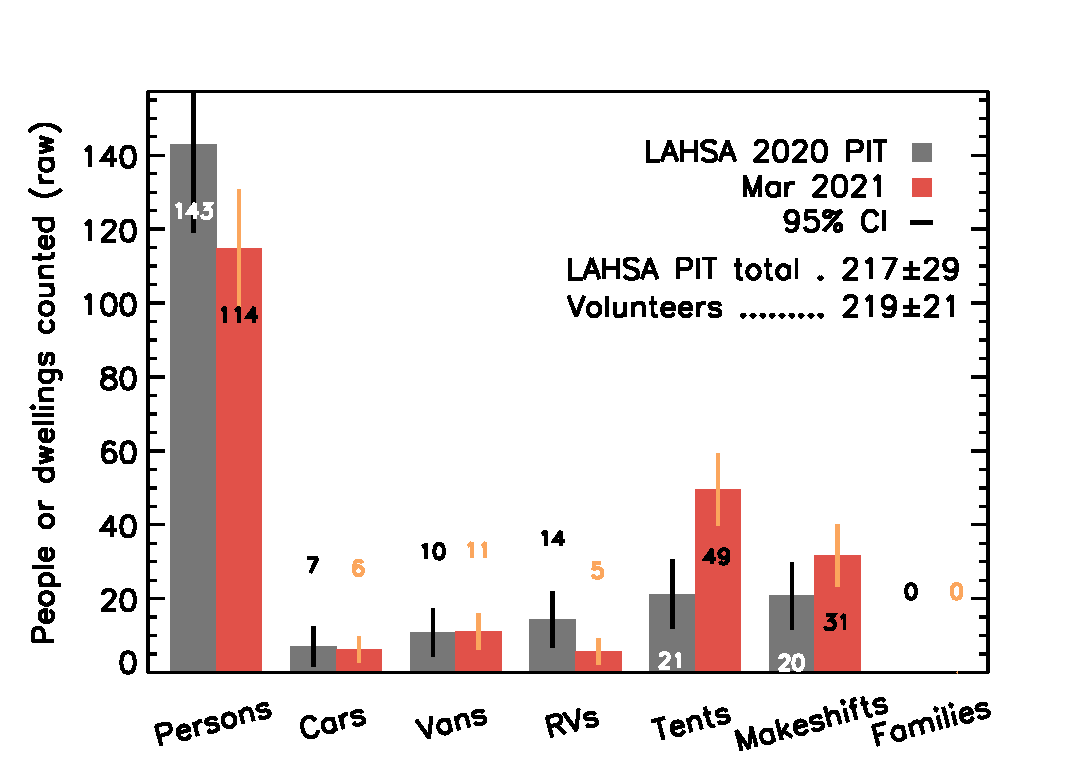
\includegraphics[width = 0.47\textwidth, trim = 1cm 0cm 0cm 1cm]{bars}
	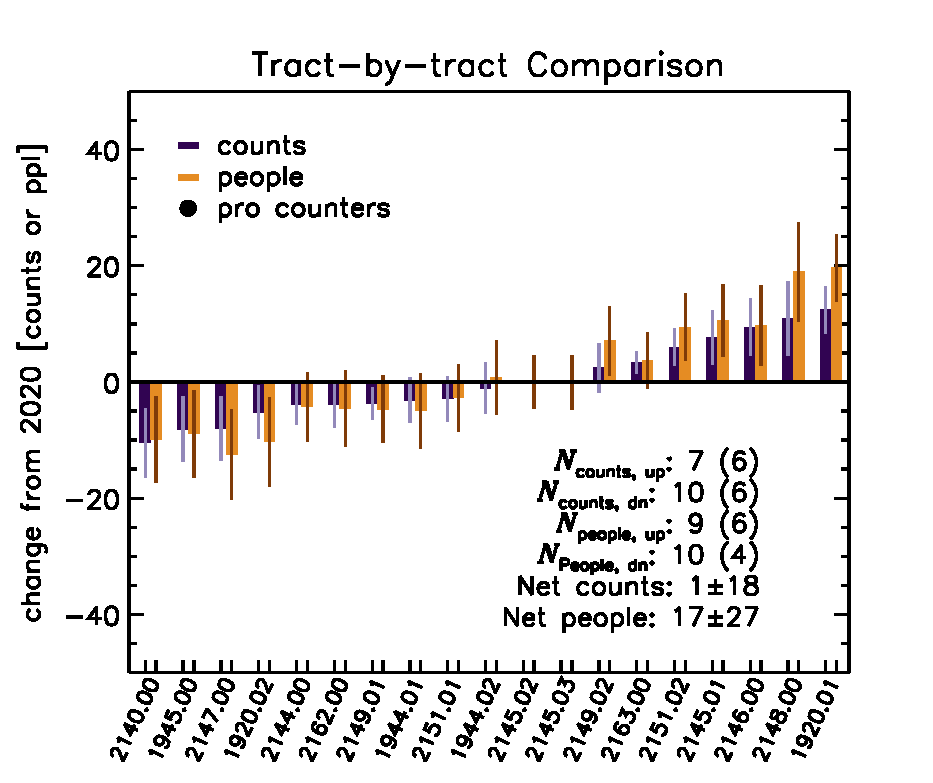
\includegraphics[width = 0.47\textwidth, trim = 0cm 0cm 0cm 1cm]{tractsYrYr.eps}	
	\caption{{\it Left:} total tallies of unsheltered persons + dwellings in Mid City West from 
			the 2020 and 2021 PIT counts (grey/colors). Persons ans RVs fell while 
			tents and perhaps makeshift structures rose. Overall, the same number of 
			people + dwellings were identified as in 2020. {\it Right:} Tract-level
			results (see also Table \ref{tbl:allTracts}). Compared to 2020, 6 tracts 
			added significantly more unsheltered people,
			4 lost them. Tracts on the Hollywood border saw the biggest changes, 
			with 2140.00's 10-person decline offset by a $\sim$20 person rise in its
			immediate northern neighbor, 1920.01.}
			%``Persons'' are TAY+Adults.
	\label{fig:rawCounts}
\end{figure*}

%\pagebreak

\noindent {\bf Context:} To compensate for the 
\href{https://laist.com/latest/post/20201209/LAHSA-cancels-2021-homeless-count-los-angeles-covid-19}
{cancellation} of the 2021 LAHSA Count, volunteer organizations in Mid City 
West\footnote{{\bfr ORGS} and resident organizers.} conducted a grassroots enumeration of 
people experiencing unsheltered homelessness 
in all 19 census tracts comprising that community on March 31, 2021 (Figure \ref{fig:tcomp}).\\

\begin{wrapfigure}{r}{0.625\linewidth}
	\centering
	\includegraphics[width=\linewidth, trim = 0cm 0cm 0cm 0cm]{map}
	\caption{The count area with census tracts colored by  
			changes in unsheltered population from 2020 (red$+$, blue$-$).
			Tracts 2140.00 and 1920.01 saw the largest changes, with the former losing
			10 people and the latter rising by 20. 
			Explore the data at \url{https://pit.demoply.org}.}
	\label{fig:tcomp}
\end{wrapfigure} 

\noindent {\bf Results:} The population estimates in Table \ref{tbl:summary} reflect all 
people, cars, vans, RVs, tents, and makeshift structure seen that night with each
dwelling weighted by its average occupancy. The latter are defined by the area-weighted 
average of the weights in the LAHSA-defined 
\href{https://www.lahsa.org/documents?id=4686-2020-greater-los-angeles-city-community-homelessness-report-service-planning-area-4.pdf}{communities} of Fairfax (30\%), Mid Wilshire (30\%), and 
Beverly Grove (40\%) from which Mid City West is constituted. Results are unchanged if 
the \href{https://www.lahsa.org/documents?id=4635-usc-2018-2020-multipliers-and-estimates-overview}
{SPA4/CD5} or \href{https://www.lahsa.org/documents?id=4693-2020-greater-los-angeles-homeless-count-cvrtm-conversion-factors}{SPA4-wide} occupancies are used instead, or if the tent weight is 
updated based on a March survey performed by {\it The People Concern}.\footnote{Outreach teams 
assessed that 52 people occupied 39 surveyed tents in or around the Mid City West Community,
yielding an estimated $1.33\pm0.18$ people per tent vs.~LAHSA's 2020 value of $1.49\pm0.11$.}

Most formally, from 10,000 simulations based on the results of the Mid City Count, 22 out of 100 surveys 
would find an unsheltered population lower than 2020's (Figure \ref{fig:hist}). This probability is too 
high compared to the 5 out of 100 benchmark to support claims that the observed 7\% increase is real.

\begin{wrapfigure}{r}{0.625\linewidth}
	\centering
	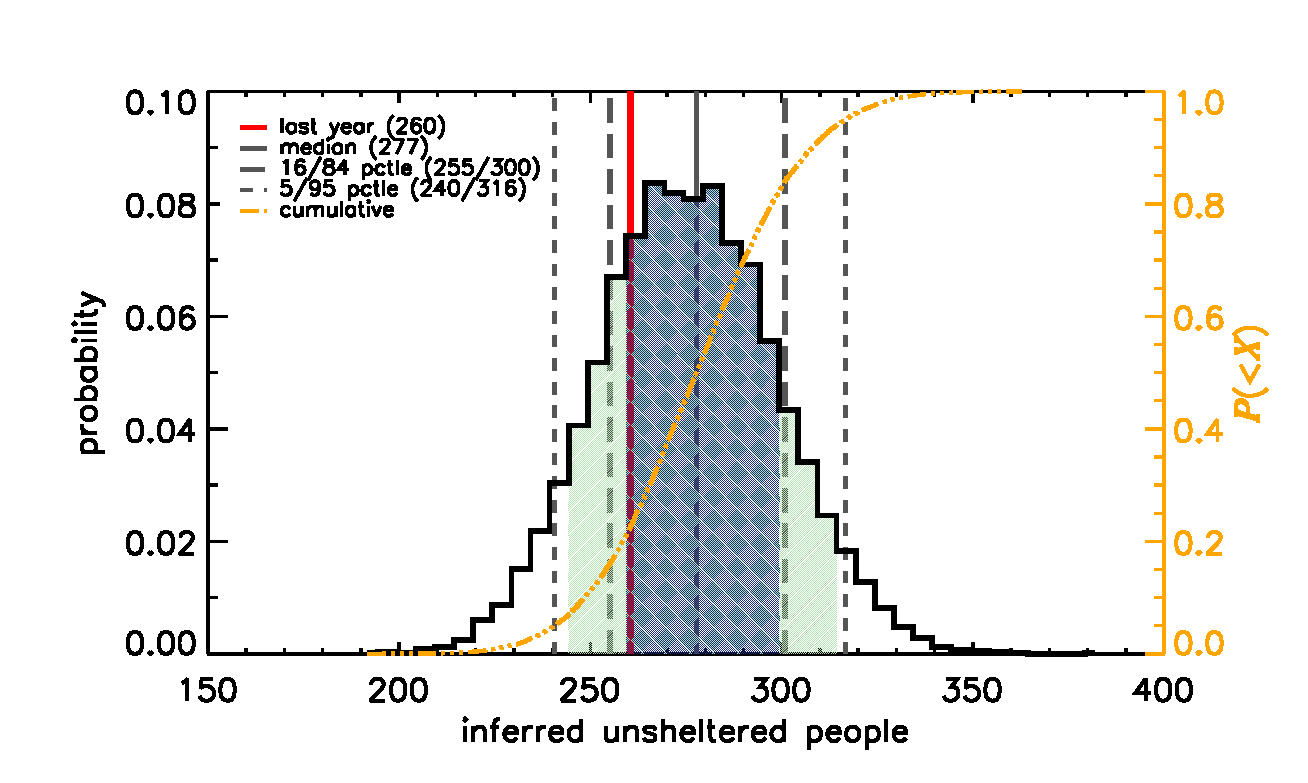
\includegraphics[width=\linewidth, trim = 0cm 0cm 0cm 0cm]{mcw2021Hist}
	\caption{Probability distributions for the total unsheltered population in Mid City West.}
	\label{fig:hist}
\end{wrapfigure} 

Given turnout, 14 out of 19 total tracts were counted at least twice (Table \ref{tbl:allTracts}). 
Comparisons of total and per-category counts by those tracts' independent surveyors
suggests that visual tally errors are consistent with the random mistakes already accounted for 
in the above analysis. The total count uncertainty is 10\% (95\% CI) with the remainder 
of the 15\% total population error due to uncertainties in dwelling occupancies.\\

\begin{table}[b]
\caption{Census Tract-level Unsheltered Data}
%\resizebox{\textwidth}{!}{%
\centering
\begin{tabular}{ccccc}
\toprule
Tract & Counter & Passes & Median Est. & 90\% CI \\ \cmidrule{1-5}
1920.01 & Vol & 3 & 29 & 21--37 \\
1920.02 & Vol & 2 & 13 & 5--20 \\
1944.01 & Vol & 2 & 10 & 2--17 \\
1944.02 & Vol & 2 & 16 & 8--23 \\
1945.00 & Vol & 2 & 19 & 10--26 \\
2140.00 & Vol & 2 & 19 & 11--27 \\
2144.00 & Vol & 2 & 6 & 0--14 \\
2145.01$^{\rm a}$ & Pro/Vol & 2 & 24 & 15--31 \\
2145.02 & Vol & 1 & 0 & 0--7 \\
2145.03 & Vol & 1 & 0 & 0--7 \\
2146.00 & Vol & 2 & 27 & 19--34 \\
2147.00 & Vol & 1 & 12 & 3--19 \\
2148.00 & Vol & 2 & 46 & 36--56 \\
2149.01 & Vol & 3 & 4 & 0--11 \\
2149.02 & Vol & 2 & 19 & 10--26 \\
2151.01 & Vol & 1 & 7 & 0--14 \\
2151.02 & Vol & 1 & 11 & 2--20 \\
2162.00 & Vol & 2 & 10 & 2--18 \\
2163.00 & Vol & 3 & 6 & 0--13 \\
\cmidrule{1-5}
{\bf All} & & {\bf 36} & {\bf 277} & {\bf 240--316}
\\ \bottomrule
\end{tabular}
%}
\caption*{$^{\rm a}$Pan Pacific Park counted by professional outreach teams
31 March and volunteers 14 April; home to known emergency shelter.}
\label{tbl:allTracts}
\end{table}

\noindent {\bf Comments:} The change we find mainly reflects a $\sim$30\% drop in the raw number
of adult individuals seen on the street. This fact has caused the total number of unsheltered people to shrink 
even as tents more than doubled in 28\% of tracts. Government initiatives to stop evictions and move 
people indoors and may be responsible. If \href{https://www.lahsa.org/documents?id=4672-2020-homeless-count-council-district-13}{CD13's} 6.5\% share of \href{https://www.lahsa.org/documents?id=4585-2020-greater-los-angeles-homeless-count-los-angeles-continuum-of-care-coc-}{LA County's unsheltered seniors} 
is an indication, 100 Greater Hollywood residents might have been in any of Project Roomkey's 
\href{https://projectroomkeytracker.com/}{1608 active rooms} on the night of the count---about half the 
inferred change. The new Riverside \href{https://www.lamayor.org/ABridgeHome}
{\it A Bridge Home} and 120 PATH supportive housing units may also have contributed.
Coordinated Entry System data will show if the above scenarios are true.

If there are fewer people on the street, however, their quality of life is worse. 
COVID has restricted or eliminated access to restaurant bathrooms, libraries 
(\href{https://www.lapl.org/homeless-resources/the-source}{\it The Source}), DPSS 
(EBT, Medi-Cal), DMV (IDs), and DMH facilities. Physical limits on client access at 
hospitals has also kept caseworkers from managing successful discharges. These harms 
are reflected by a 25\% increase in 
\href{https://www.latimes.com/california/story/2021-01-07/the-powerful-synthetic-opioid-fentanyl-is-behind-rising-deaths-in-the-homeless-population}{overdose deaths} and made more visible by \href{https://clkrep.lacity.org/onlinedocs/2020/20-0147_misc_3-17-20_p.pdf}{suspended}
tent folding and sanitation practices as tents increased in many places. 
Of course, a decline of just 12\% means substantial coming challenges
 \href{https://www.latimes.com/california/story/2021-01-12/new-report-foresees-tens-of-thousands-losing-homes-by-2023}
{as eviction moratoriums lapse}.

If our data support the effectiveness of programs aimed at reducing street homelessness, 
they do {\it not} suggest that the state of homelessness has improved. In the fight to rebuild lives---as well 
as build homes---that fact must remain paramount.

Learn more about the count at \url{https://hollywood4wrd.live/2021-homeless-count}.

%\clearpage

\end{document}  